\documentclass[8pt,a4paper,compress,handout]{beamer}

\usepackage{/home/siyer/lib/slides}

\title{Recursion}
\date{}

\begin{document}
\begin{frame}
\hfill
\begin{minipage}{150pt}
\begin{flushright}
\tiny \emph{To iterate is human, to recurse divine.}

\smallskip

- L. Peter Deutsch
\end{flushright}
\end{minipage}
\titlepage
\end{frame}

\begin{frame}
\frametitle{Outline}
\tableofcontents
\end{frame}

\section{What is Recursion?}
\begin{frame}[fragile]
A \emph{recursive function} is a function that calls itself and meets the following conditions:
\begin{itemize}
\item Has a \emph{base case}; 
\item Addresses subproblems that are \emph{smaller} in some sense; and
\item Does not address subproblems that \emph{overlap}.
\end{itemize}

\bigskip

Recursive programming is directly related to \emph{mathematical induction}, a technique for proving facts about discrete functions.
\end{frame}

\section{Examples}
\begin{frame}[fragile]
Recursive definition of the factorial function $N!$ and its implementation in Python: 
\[
N! = \begin{dcases*}
N(N-1)! & if $N > 0$, and \\
1       & if $N=0$.
\end{dcases*}
\]

\begin{lstlisting}[language=Python]
def factorial(N):
    if N == 0:
        return 1
    return N * factorial(N - 1)
\end{lstlisting}

\bigskip

Call trace for \lstinline{factorial(5)}:
\begin{lstlisting}[language={}]
factorial(5)
  factorial(4)
    factorial(3)
      factorial(2)
        factorial(1)
          return 1
        return 2 * 1 = 2
      return 3 * 2 = 6
    return 6 * 4 = 24
  return 24 * 5 = 120
\end{lstlisting}
\end{frame}

\begin{frame}[fragile]
Recursive definition of the $n$th harmonic number $H_n$ and its implementation in Python: 
\[
H_n = \begin{dcases*}
\frac{1}{n} + H_{n-1} & if $n > 1$, and \\
1       & if $n=1$.
\end{dcases*}
\]

\begin{lstlisting}[language=Python]
def harmonic(n):
    if n == 1:
        return 1.0
    return 1.0 / n * harmonic(n - 1)
\end{lstlisting}

\bigskip

Call trace for \lstinline{harmonic(5)}:
\begin{lstlisting}[language={}]
harmonic(5)
  harmonic(4)
    harmonic(3)
      harmonic(2)
        harmonic(1)
          return 1.0
        return 1.0 / 2 + 1.0 = 1.5
      return 1.0 / 3 + 1.5 = 1.8333333333333333
    return 1.0 / 4 + 1.8333333333333333 = 2.083333333333333
  return 1.0 / 5 + 2.083333333333333 = 2.283333333333333
\end{lstlisting}
\end{frame}

\begin{frame}[fragile]
\begin{framed}
\tiny euclid.py: Accept integers $p$ and $q$ as command-line arguments, compute the greatest common divisor of $p$ and $q$, and write the result to standard output.
\end{framed}

\begin{lstlisting}[language=Python]
import stdio
import sys

def gcd(p, q):
    if q == 0:
        return p
    return gcd(q, p % q)

def main():
    p = int(sys.argv[1])
    q = int(sys.argv[2])
    divisor = gcd(p, q)
    stdio.writeln(divisor)

if __name__ == '__main__':
    main()
\end{lstlisting}

\begin{lstlisting}[language={}]
$ python euclid.py 1440 408
24
$ python euclid.py 314159 271828
1
\end{lstlisting}
\end{frame}

\begin{frame}[fragile]
Call trace for \lstinline{gcd(1440, 408)}:

\begin{lstlisting}[language={}]
gcd(1440, 408)
  gcd(408, 216)
    gcd(216, 192)
      gcd(192, 24)
        gcd(24, 0)
          return 24
        return 24
      return 24
    return 24
  return 24
\end{lstlisting}
\end{frame}

\begin{frame}[fragile]
\begin{framed}
\tiny towersofhanoi.py: Accept integer $n$ as a command-line argument. Write to standard output instructions to move $n$ Towers of Hanoi disks to the left.
\end{framed}

\begin{lstlisting}[language=Python]
import stdio
import sys

def moves(n, left):
    if n == 0:
        return
    moves(n - 1, not left)
    if left:
        stdio.writeln(str(n) + ' left')
    else:
        stdio.writeln(str(n) + ' right')
    moves(n - 1, not left)

def main():
    n = int(sys.argv[1])
    moves(n, True)

if __name__ == '__main__':
    main()
\end{lstlisting}

\begin{lstlisting}[language={}]
$ python towersofhanoi.py 3
1 left
2 right
1 left
3 left
1 left
2 right
1 left
\end{lstlisting}
\end{frame}

\begin{frame}[fragile]
\begin{lstlisting}[language={}]
$ python towersofhanoi.py 4
1 right
2 left
1 right
3 right
1 right
2 left
1 right
4 left
1 right
2 left
1 right
3 right
1 right
2 left
1 right
\end{lstlisting}
\end{frame}

\begin{frame}[fragile]
Call trace for \lstinline{moves(4, True)}:

\begin{lstlisting}[language={}]
moves(4, True)
  moves(3, False)
    moves(2, True)
      moves(1, False)
        1 right
      2 left
      moves(1, False)
        1 right
    3 right
    moves(2, True)
      moves(1, False)
        1 right
      2 left
      moves(1, False)
        1 right
  4 left
  moves(3, False)
    moves(2, True)
      moves(1, False)
        1 right
      2 left
      moves(1, False)
        1 right
    3 right
    moves(2, True)
      moves(1, False)
        1 right
      2 left
      moves(1, False)
        1 right
\end{lstlisting}
\end{frame}

\begin{frame}[fragile]
\begin{framed}
\tiny beckett.py: Accept integer $n$ as a command-line argument. Write to standard output Beckett's stage instructions for $n$ actors.
\end{framed}

\begin{lstlisting}[language=Python]
import stdio
import sys

def moves(n, enter):
    if n == 0:
        return
    moves(n - 1, True)
    if enter:
        stdio.writeln('enter ' + str(n))
    else:
        stdio.writeln('exit  ' + str(n))
    moves(n - 1, False)

def main():
    n = int(sys.argv[1])
    moves(n, True)

if __name__ == '__main__':
    main()
\end{lstlisting}

\begin{lstlisting}[language={}]
$ python beckett.py 3
enter 1
enter 2
exit  1
enter 3
enter 1
exit  2
exit  1
\end{lstlisting}
\end{frame}

\begin{frame}[fragile]
\begin{framed}
\tiny htree.py: Accept integer $n$ as a command-line argument. Draw a level $n$ H-tree centered at $(.5, .5)$ with lines of length $.5$.
\end{framed}

\begin{lstlisting}[language=Python]
import stddraw
import sys

def draw(n, lineLength, x, y):
    if n == 0:
        return
    x0 = x - lineLength / 2
    x1 = x + lineLength / 2
    y0 = y - lineLength / 2
    y1 = y + lineLength / 2
    stddraw.line(x0, y, x1, y)
    stddraw.line(x0, y0, x0, y1)
    stddraw.line(x1, y0, x1, y1)
    draw(n - 1, lineLength / 2, x0, y0)
    draw(n - 1, lineLength / 2, x0, y1)
    draw(n - 1, lineLength / 2, x1, y0)
    draw(n - 1, lineLength / 2, x1, y1)

def main():
    n = int(sys.argv[1])
    stddraw.setPenRadius(0.0)
    draw(n, .5, .5, .5)
    stddraw.show()

if __name__ == '__main__':
    main()
\end{lstlisting}
\end{frame}

\begin{frame}[fragile]
\begin{minipage}{160pt}
\begin{lstlisting}[language={}]
$ python htree.py 1
\end{lstlisting}
\end{minipage}%
\begin{minipage}{140pt}
\hfill 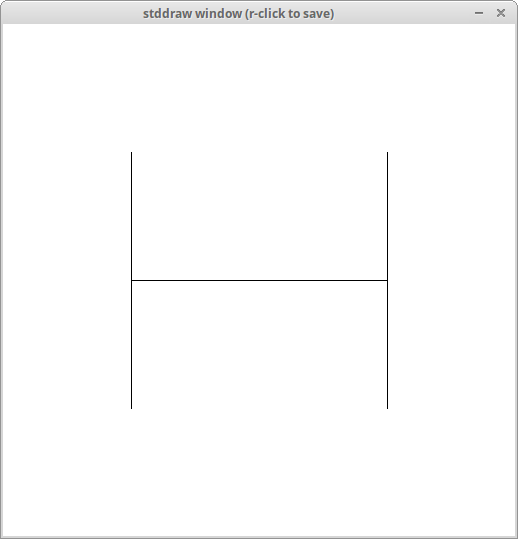
\includegraphics[scale=0.15]{figures/htree1.png}
\end{minipage}

\smallskip

\begin{minipage}{160pt}
\begin{lstlisting}[language={}]
$ python htree.py 3
\end{lstlisting}
\end{minipage}%
\begin{minipage}{140pt}
\hfill 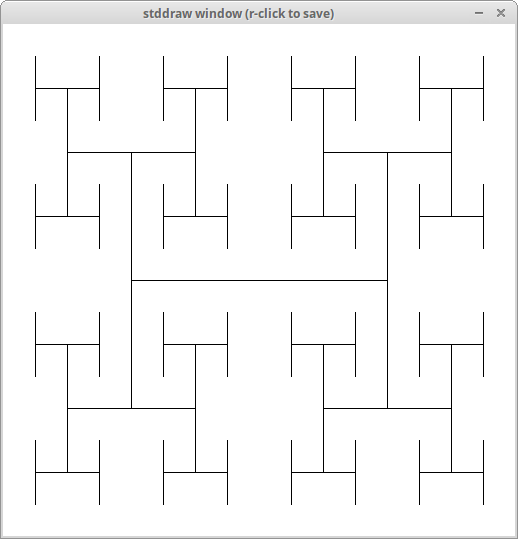
\includegraphics[scale=0.15]{figures/htree2.png}
\end{minipage}

\smallskip

\begin{minipage}{160pt}
\begin{lstlisting}[language={}]
$ python htree.py 5
\end{lstlisting}
\end{minipage}%
\begin{minipage}{140pt}
\hfill 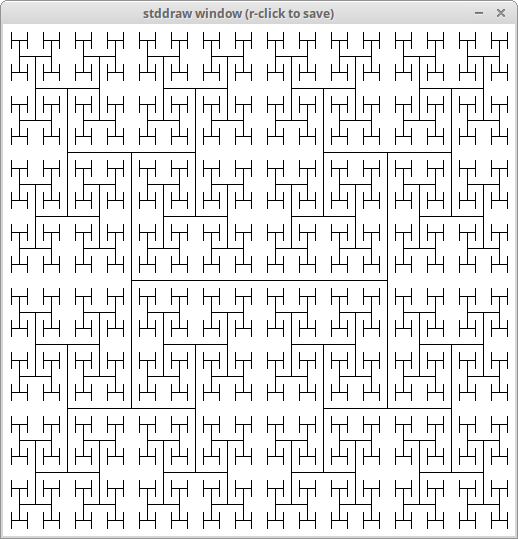
\includegraphics[scale=0.15]{figures/htree3.png}
\end{minipage}
\end{frame}

\begin{frame}[fragile]
\begin{framed}
\tiny brownian.py: Accept a Hurst exponent as a command-line argument. Use the Hurst exponent to compute a scale factor. Draw a Brownian bridge from $(0, .5)$ to $(1.0, .5)$ with variance $.01$ and that scale factor.
\end{framed}

\begin{lstlisting}[language=Python]
import math
import stddraw
import stdrandom
import sys

def curve(x0, y0, x1, y1, variance, scaleFactor):
    if (x1 - x0) < .01:
        stddraw.line(x0, y0, x1, y1)
        return
    xm = (x0 + x1) / 2.0
    ym = (y0 + y1) / 2.0
    delta = stdrandom.gaussian(0, math.sqrt(variance))
    curve(x0, y0, xm, ym + delta, variance / scaleFactor, scaleFactor)
    curve(xm, ym + delta, x1, y1, variance / scaleFactor, scaleFactor)

def main():
    hurstExponent = float(sys.argv[1])
    stddraw.setPenRadius(0.0)
    scaleFactor = 2 ** (2.0 * hurstExponent)
    curve(0, .5, 1.0, .5, .01, scaleFactor)
    stddraw.show()

if __name__ == '__main__':
    main()
\end{lstlisting}
\end{frame}

\begin{frame}[fragile]
\begin{minipage}{160pt}
\begin{lstlisting}[language={}]
$ python brownian.py 1
\end{lstlisting}
\end{minipage}%
\begin{minipage}{140pt}
\hfill 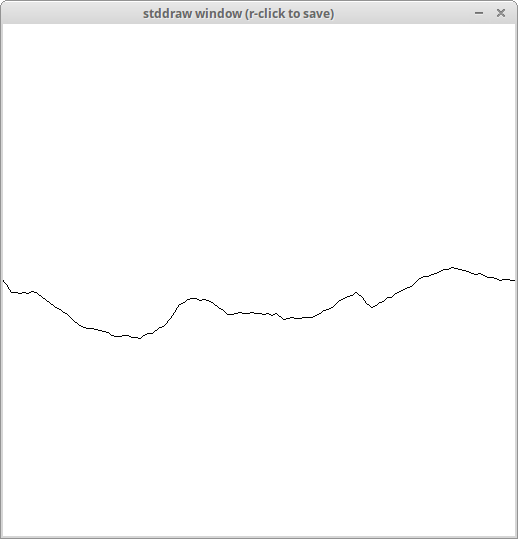
\includegraphics[scale=0.15]{figures/brownian1.png}
\end{minipage}

\smallskip

\begin{minipage}{160pt}
\begin{lstlisting}[language={}]
$ python brownian.py .5
\end{lstlisting}
\end{minipage}%
\begin{minipage}{140pt}
\hfill 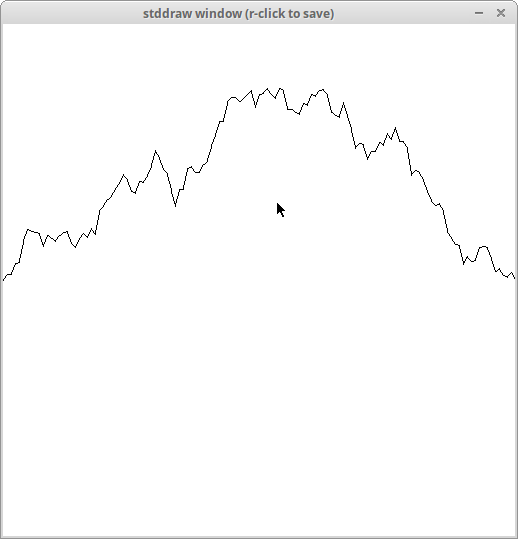
\includegraphics[scale=0.15]{figures/brownian2.png}
\end{minipage}

\smallskip

\begin{minipage}{160pt}
\begin{lstlisting}[language={}]
$ python brownian.py .05
\end{lstlisting}
\end{minipage}%
\begin{minipage}{140pt}
\hfill 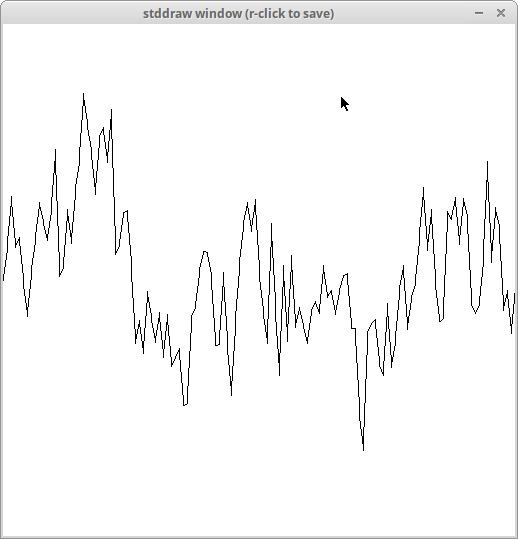
\includegraphics[scale=0.15]{figures/brownian3.png}
\end{minipage}
\end{frame}

\section{Pitfalls}
\begin{frame}[fragile]
Missing base case. 
\begin{lstlisting}[language=Python]
def harmonic(n):
    return 1.0 / n + harmonic(n - 1)
\end{lstlisting}

\bigskip

Recursion does not address \emph{smaller} subproblems.
\begin{lstlisting}[language=Python]
def harmonic(n):
    if n == 1: 
        return 1.0
    return 1.0 / n + harmonic(n)
\end{lstlisting}

\bigskip

Recursion addresses \emph{overlapping} subproblems.
\begin{lstlisting}[language=Python]
def fibonacci(n):
    if n == 0 or n == 1:
        return n
    return fibonacci(n - 1) + fibonacci(n - 2)  
\end{lstlisting}

\bigskip

If a function calls itself recursively an excessive number of times before returning, the memory required by Python to keep track of the recursive calls may be prohibitive, resulting in a runtime error. 
\end{frame}
\end{document}
